\subsection{The pbdR Project}


\begin{frame}
  \begin{block}{Programming with Big Data in R (pbdR)}
       \centering Striving for \emph{Productivity, Portability, Performance}\\[.4cm]\pause
  \begin{columns}[onlytextwidth]
    \begin{column}{0.30\textwidth}
      \centering
       
\includegraphics[width=3.4cm]{../common/pics/simple}\\[.2cm]
    \end{column}
    \begin{column}{0.65\textwidth}
  \begin{itemize}[<+-|alert@+>]
    \item \emph{Free}\footnote{MPL, BSD, and GPL licensed} R packages.
    \item Bridging high-performance compiled code with high-productivity of R
    \item Scalable, big data analytics.
    \item Offers implicit and explicit parallelism.
    \item Methods have syntax \emph{identical} to R.
  \end{itemize}
    \end{column}
​  \end{columns}
\end{block}
\end{frame}




\begin{frame}
  \begin{block}{pbdR Packages}
    \begin{center}
%         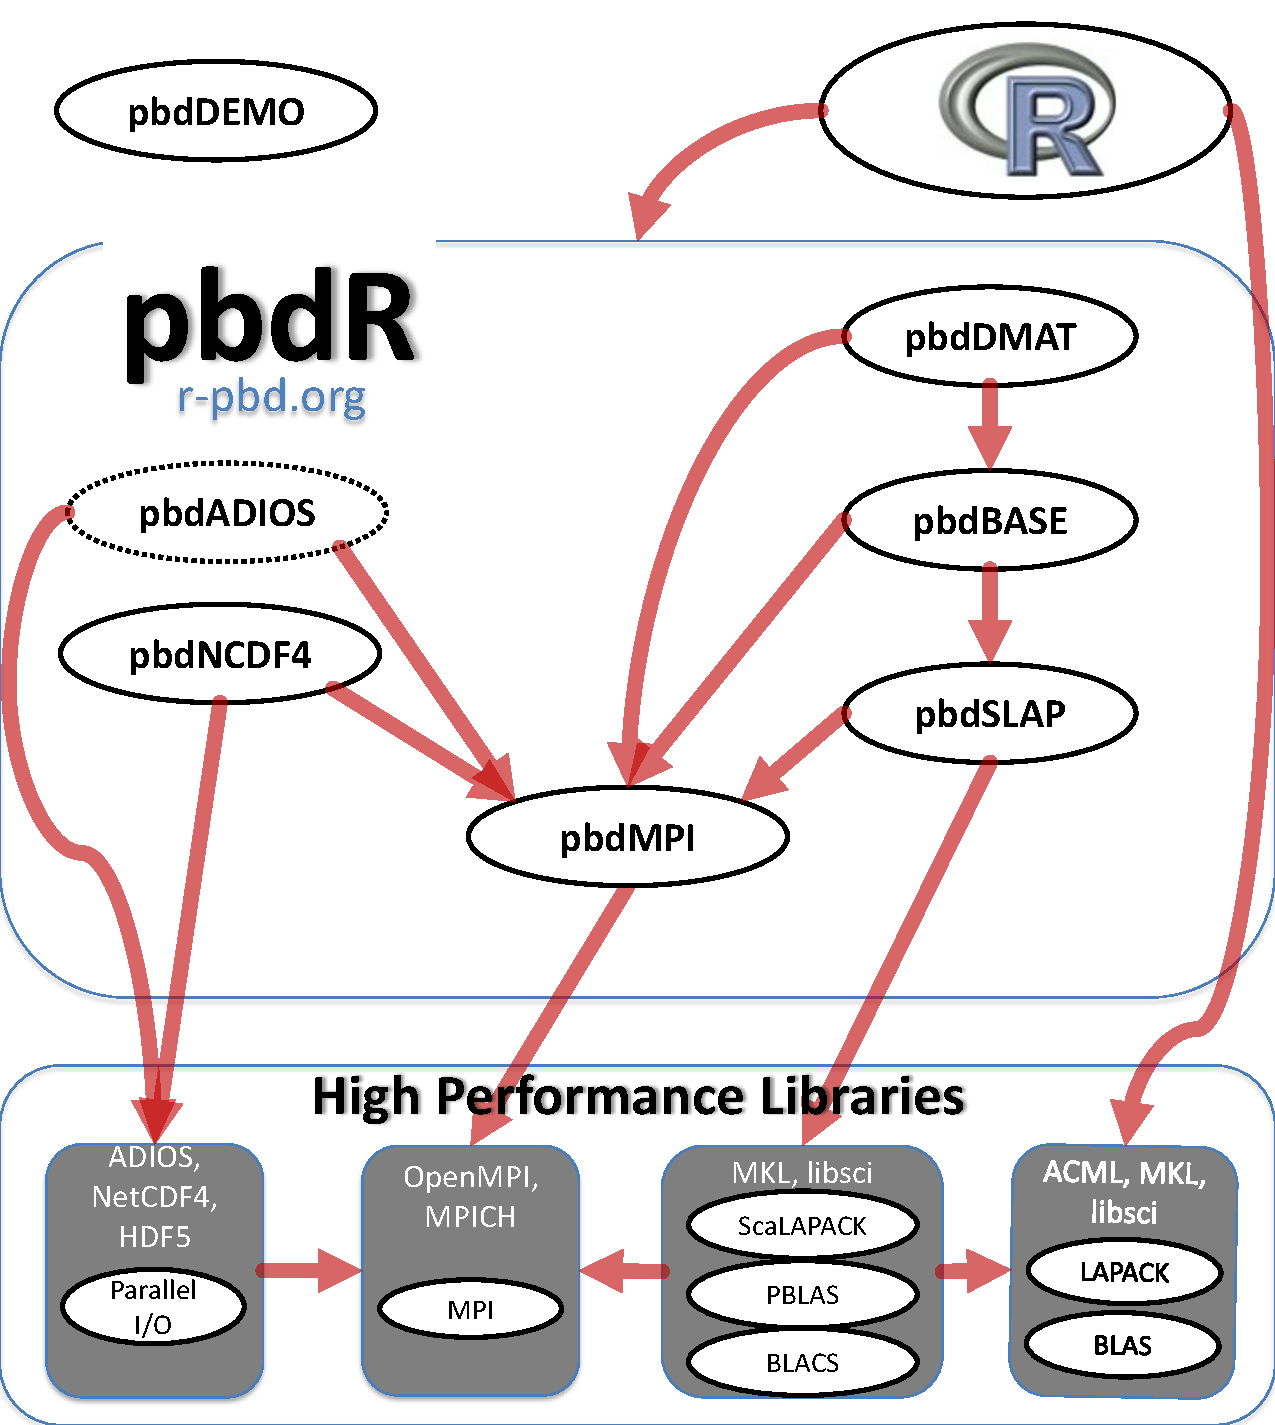
\includegraphics[width=7cm, height=7cm]{pics/pbdpacks}
      \begin{columns}
        \begin{column}{.52\textwidth}
      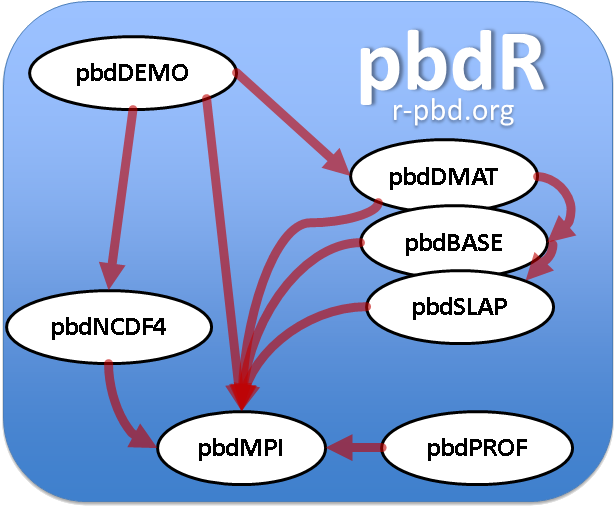
\includegraphics[scale=.4]{../common/pics/pbdR}
        \end{column}
        \hspace{.05cm}
        \begin{column}{.4\textwidth}
      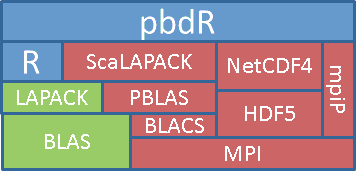
\includegraphics[scale=.45]{../common/pics/libs}
        \end{column}
      \end{columns}
    \end{center}
  \end{block}
\end{frame}


%%% MPI
% \begin{frame}[fragile]
%   \begin{block}{Simple, Intuitive MPI Operations with \textbf{pbdMPI}}\pause
%   \begin{center}
%  \begin{minipage}{.9\textwidth}
%  \centering\vspace{-.55cm}
% \begin{lstlisting}[title=\ ,basicstyle=\scriptsize,numbers=none]
% Placeholder
% \end{lstlisting}
%  \end{minipage}
%  \end{center}
%   \end{block}
% \end{frame}


%%% DMAT/BASE/SLAP
\begin{frame}[fragile]
  \begin{block}{Distributed Matrices and Statistics with \textbf{pbdDMAT}}\pause
  \begin{center}
  \begin{minipage}{.9\textwidth}
  \centering\vspace{-.1cm}
	Least Squares Benchmark
		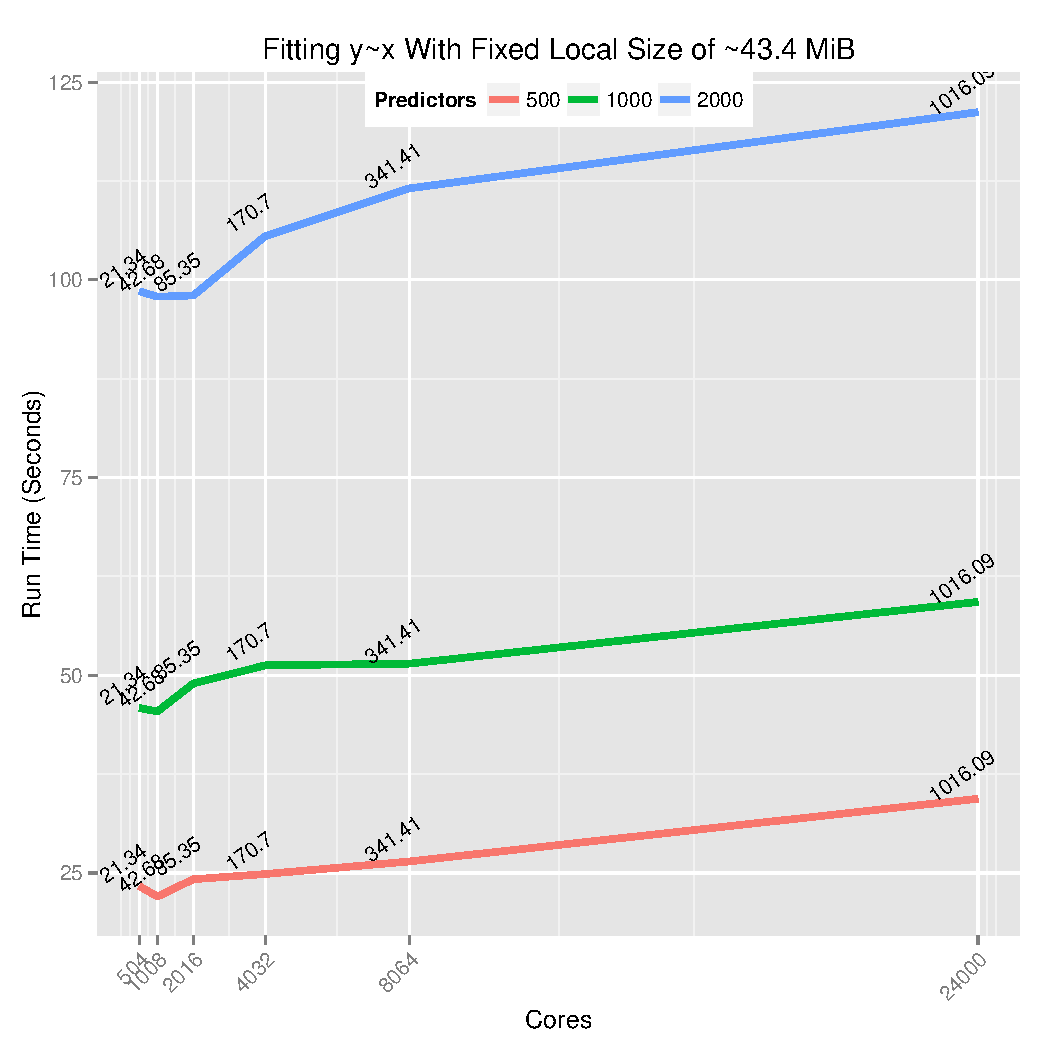
\includegraphics[width=7cm,height=5.75cm]{../common/pics/benchmarks/lmfit2}
  \end{minipage}
 \begin{minipage}{.9\textwidth}
 \centering\vspace{-.55cm}
\begin{lstlisting}[title=\ ,basicstyle=\scriptsize,numbers=none]
x <- ddmatrix("rnorm", nrow=m, ncol=n)
y <- ddmatrix( "rnorm", nrow=m, ncol=1)
mdl <- lm.fit(x=x, y=y)
\end{lstlisting}
 \end{minipage}
 \end{center}
  \end{block}
\end{frame}



%%% PROF
\begin{frame}[fragile]
  \begin{block}{Profiling with \textbf{pbdPROF}}
  \begin{minipage}[t]{.58\textwidth}
  \vspace{0pt}
  1. Rebuild \pbdR\ packages
\vspace*{-.5cm}
\begin{lstlisting}[language=shl,title=\ ]
R CMD INSTALL pbdMPI_0.2-1.tar.gz \ --configure-args= \ "--enable-pbdPROF"
\end{lstlisting}
\vspace{.15cm}
2. Run code
\vspace*{-.5cm}
\begin{lstlisting}[language=shl,title=\ ]
mpirun -np 64 Rscript my_script.R
\end{lstlisting}
\vspace{.15cm}
3. Analyze results
\vspace{-.5cm}
\begin{lstlisting}[title=\ ]
library(pbdPROF)
prof <- read.prof( "profiler_output.mpiP")
plot(prof)
\end{lstlisting}
  \end{minipage}
  \hfill
  \begin{minipage}[t]{.4\textwidth}
  \vspace{0pt}
    \centering
    Publication-quality graphs\\
    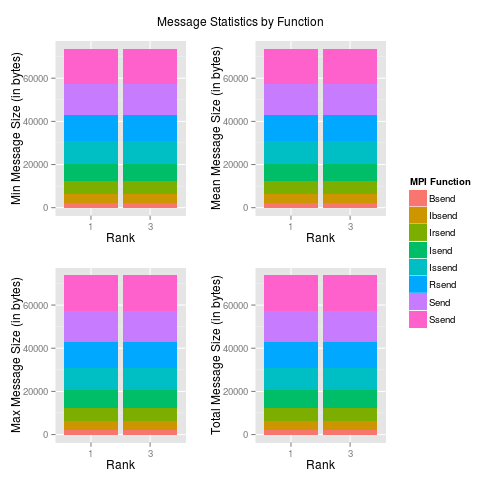
\includegraphics[scale=.25]{../common/pics/mpip}
    \\[.1cm]
    
\includegraphics[scale=0.4]{../common/pics/gsoc}
  \end{minipage}
  \end{block}
\end{frame}

